\section{Discretized Radiative Transfer Equation}
\label{sec:discretized_rte}

Our method derives from the radiative transfer equation (RTE), which expresses the change of the radiance field $L$, with respect to an infinitesimal change of position in direction $\omega$ at point $\vec{x}$:
\begin{align}
%\label{eq:rte}
\left(\nabla\cdot\omega\right)L\left(\vec{x}, \omega \right)
=&
-\sigma_t\left(\vec{x}\right) L\left(\vec{x}, \omega \right)\nonumber\\
&
+\sigma_s\left(\vec{x}\right) \int_{\Omega}
{
p\left(\omega'\cdot\omega\right)L\left(\vec{x}, \omega' \right)\ud\omega'
}\nonumber\\
&
+Q\left(\vec{x}, \omega\right)\nonumber
\  .
\label{eq:rte}
\end{align}

The left hand side (LHS) is the transport term, and we refer to the terms on the right hand side (RHS) as collision, scattering, and source term, respectively. The symbols $\sigma_t$, $\sigma_s$, $p$, and $Q$ refer to the extinction- and scattering coefficient, phase function and emission.

The RTE is often given in operator notation, where transport, collision, and scattering are expressed as operators $\mathcal{T}$, $\mathcal{C}$ and $\mathcal{S}$, which are applied to the radiance field $L$:
\begin{align}
\mathcal{T}\left(L\right) = -\mathcal{C}\left(L\right) + \mathcal{S}\left(L\right) + Q
\ .
\end{align}

Deterministic methods are derived by discretizing the angular and spatial domain. This gives rise to a linear system of equations, which can be solved using standard methods. For the $P_N$-method, the angular variable is first discretized, using a truncated spherical harmonics expansion. This results in the $P_N$-equations, a system of coupled PDEs that still depend on a continuous spatial variable.

The number of equations grows with the truncation order $N$. This is why the discretization is laborious and difficult to do without errors if done by hand. We therefore use a computer algebra representation to automate this process. After giving an outline of the general discretization in this section, we will present our computer algebra representation in the next section. The $P_N$-equations that result from our automated discretization are given in Section~\ref{sec:real_valued_pn_eq}. 

Since the radiance field $L$ is real, we use the real-valued SH basis functions $\SHBR^{l,m}$, which are defined in terms of the complex-valued SH basis functions $\SHBC^{l,m}$:
\begin{align}
\SHBR^{l,m}=
\left\{
\begin{array}{lr}
\frac{\iu}{\sqrt{2}}\left(\SHBC^{l,m}-\left(-1\right)^m\SHBC^{l,-m}\right), & \text{for } m < 0\\
\SHBC^{l,m}, & \text{for } m = 0\\
\frac{1}{\sqrt{2}}\left(\SHBC^{l,-m}-\left(-1\right)^m\SHBC^{l,m}\right), & \text{for } m > 0
\end{array}
\right.
\label{eq:sh_real_basis}
\end{align}

We express the projection into the spherical harmonics basis functions with a projection operator $\mathcal{P}$:
\begin{align}
\mathcal{P}^{l, m}(f) = \int_{\Omega}f(\vec{x}, \omega) \SHBR^{l,m}(\omega)\,\mathrm{d}\omega = f^{l,m}\left(\vec{x}\right)
\ .
\nonumber
\end{align}

The $P_N$-equations are derived by first expressing all direction-dependent parameters in spherical harmonics. The radiance field $L$ in Equation~\ref{eq:rte} is therefore replaced by its SH reconstruction $\widehat{L}$, introducing an error due to truncation at order $N$:
\begin{align}
\widehat{L}\left(\vec{x}, \omega\right) =
\sum_{l=0}^{N}
{
\sum_{m=-l}^{l}
{
L^{l,m}\left(\vec{x}\right)\SHBR^{l,m}\left(\omega\right)
}
}
\approx
L\left(\vec{x}, \omega\right)
\ .
\nonumber
\end{align}

\vspace{0.5in}

After substitution, all angular parameters are expressed in terms of spherical harmonics, but they still depend on the continuous angular variable $\omega$. As a next step, we project each term of the RTE into spherical harmonics, using the projection operator $\mathcal{P}$. This produces a single equation for each $l,m$-pair. The $P_N$-equations therefore can be written as:
\begin{align}
\mathcal{P}^{l,m}\mathcal{T}\left(\widehat{L}\right)
=
-\mathcal{P}^{l,m}\mathcal{C}\left(\widehat{L}\right) 
+\mathcal{P}^{l,m}\mathcal{S}\left(\widehat{L}\right)
+\mathcal{P}^{l,m}\left(Q\right)
\ .
\label{eq:pn_operator_notation}
\end{align}

Once the $P_N$-equations have been found, the spatial variable $\vec{x}$ is discretized using a finite difference (FD) voxel grid (using central differences for differential operators).

Following this discretization, the radiance field $L$, is represented as a set of SH coefficients per voxel. Flattening these over all voxels into a single vector, gives the solution vector $\vec{u}$. The RHS vector $\vec{Q}$ is produced similarly. The projected operators can be expressed as linear transformations, which can be collapsed into a single coefficient matrix $A$ (see Figure~\ref{fig:matrix_layout}):
\begin{align}
(T+C-S)\vec{u} = A\vec{u} = \vec{Q}
\ .
\end{align}

$T$, $C$, $S$ are matrices, which result from the discretized transport, collision and scattering operators respectively.

\begin{figure}[h]
\centering
%\missingfigure{test}
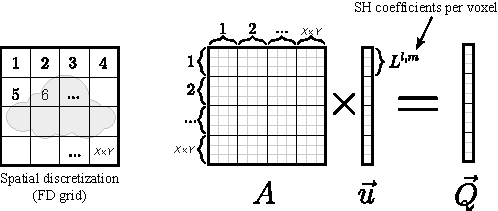
\includegraphics[width=\columnwidth]{figures/fig_matrix_layout_small.pdf}
%\missingfigure{figures fig matrix layout}
\vspace{-0.2in}
\icaption{Structure of coefficient matrix $A$ and solution vector $\vec{u}$ after discretization of the $P_N$-equations on a finite difference grid.}
\label{fig:matrix_layout}
\end{figure}

So far, we have only given the $P_N$-equations in high-level operator notation (Equation~\ref{eq:pn_operator_notation}). Carrying out the full derivation creates large, unwieldy equations and requires a string of expansions, manipulations and applications of identities. These are challenging and error-prone if done by hand. We \rev{therefore used a computer algebra representation}, which allowed us to derive and discretize the $P_N$-equation in a semi-automatic fashion.

